% #############################################################################
% This is Chapter 4
% !TEX root = ../main.tex
% #############################################################################
% Change the Name of the Chapter i the following line
\fancychapter{Related Work}
% The following line allows to ref this chapter
\label{chap:base}

\section{Automation and \ac{AI} in Regulatory Analysis and Modelling}

The evolution of \ac{RE} has undergone several transitions over the years, marked by a significant transition pivoting from traditional manual methods to more agile approaches that emphasize increased automation to reduce time, labour and human error. Early efforts in automated \ac{RE} primarily focus on the analysis phase-identified as the most widely automated phase, according to Umar and Lano \cite{Umar2024}-utilizing \ac{NLP} technologies such as Part-of-Speech tagging and syntax parsing to generate \ac{UML} models and perform consistency checks \cite{Umar2024}. However, these traditional methodologies often struggled with the nuances and ambiguities of real-world legal documents, requiring a shift toward more sophisticated \ac{AI} solutions \cite{Zadenoori2025}. 

The emergence of \ac{GenAI} and \ac{LLM}s represents a fundamental paradigm shift characterized by ``emergence'' (the ability of models to derive knowledge without explicit programming) and ``homogenization'', where a unified foundation model can tackle a wide range of specialized problems \cite{Jeong2023}. A problem arises when the model does not have sufficient information, limiting answer capabilities and creating a phenomenon called ``hallucination''. To address this issue, the \ac{RAG} model has emerged. This model stores information in databases and retrieves the necessary information to provide it to the \ac{LLM} when needed, grounding responses in specific enterprise data or legal texts \cite{Jeong2023}. Unlike \ac{NLP}, generative \ac{LLM}s synthesize and create content, allowing \ac{RE} research to focus on more ``cognitively demanding activities'', such as requirements elicitation, validation, and modelling rather than just defect detection and classification, which were dominant in the past \cite{Zadenoori2025}.

In the regulatory domain, these capabilities have enabled the development of specialized frameworks like \ac{MURCIA}. \ac{MURCIA} is ``an automated approach that leverages recent language models to assist human analysts in analysing regulatory changes.'' This approach utilizes \ac{LLM}s to navigate hundreds of legal provisions and analyse the implications of regulatory changes over time, categorizing impacts across textual, semantic, deontic, and pragmatic layers. Evaluations of this \ac{AI}-enabled approach demonstrated high efficacy, with an F1 score exceeding 90\% for identifying textual changes and text meaning \cite{Abualhaija2024}.

Additionally, research is also exploring the possibilities of a conversational approach. This approach utilizes a conceptual model interpreter where a modelling task is specified in natural language via a conversational user interface, and an \ac{LLM} generates model syntax that is automatically rendered with instant feedback. This allows for an iterative process with refinement by specifying a new modelling task. This process can be applied to \ac{RE}, and also lowers the entry barrier for modelling and design activities \cite{Haerer2023}.

Despite these advancements, a critical gap remains: current studies are often evaluated in controlled laboratory environments with limited integration into the complex, multi-regulatory workflows required in industry \cite{Zadenoori2025}. There is a ``notable absence of systematic methodologies''\cite{Elahidoost2024} that can bridge the abstraction gap between high-level regulatory extraction and the formal consolidation of these insights into an organization's enterprise architecture.

\section{\ac{LLM} Agents and Skills}

\ac{LLM}-based agents extend stand-alone language models by coupling language-based reasoning with planning, memory, tools, and interaction with an execution environment. Rather than only generating responses, an agent can interpret a goal, select actions, invoke external capabilities, observe their results, and adapt its subsequent actions accordingly \cite{ZhouEtAl2026AgentSkills}. This ability is relevant to complex modelling workflows, where the work includes information retrieval, evidence processing, structured transformation, validation, and model generation.

Recent literature distinguishes between agents and agent skills. The agent is the higher-level component responsible for interpreting intent, decomposing goals, and coordinating actions. A skill is a bounded and reusable artefact that specifies how a task should be performed under defined conditions \cite{ZhouEtAl2026AgentSkills,XuYan2026AgentSkills}. Thus, whereas a tool exposes an atomic capability, such as querying a database or producing a diagram, a skill captures the contextual knowledge required to determine when that capability should be used, how it should be sequenced with other actions, and how its outputs should be checked.

Zhou et al. conceptualise an agent skill as a tuple consisting of a primary instruction document, auxiliary resources, and applicability conditions. The auxiliary resources may include reference material, templates, schemas, executable scripts, or domain artefacts \cite{ZhouEtAl2026AgentSkills}. Xu and Yan similarly describe skills as self-contained packages that may combine a structured instruction file with supporting code, documents, and assets. This packaging allows knowledge to be externalised, inspected, reused, and revised without requiring the underlying model to be retrained \cite{XuYan2026AgentSkills}.

A central architectural principle is progressive disclosure. Skill metadata can be available for matching a task to a relevant capability, while detailed instructions and additional resources are loaded only after the skill is selected \cite{XuYan2026AgentSkills}. This reduces unnecessary context consumption and enables a larger library of specialised procedures. Skills are also complementary to tool-connectivity mechanisms such as the Model Context Protocol: such mechanisms provide access to external tools and data sources, whereas skills provide the procedural guidance for using them reliably within a workflow \cite{XuYan2026AgentSkills}.

Skills may be authored by domain experts, derived from experience or task traces, retrieved from a repository, composed for more complex workflows, and subsequently revised or retired. However, the literature also identifies open concerns regarding portability, skill selection at scale, composition, testing, provenance, permissions, and security \cite{ZhouEtAl2026AgentSkills,XuYan2026AgentSkills}. These concerns are especially relevant where skills operate on legally significant sources or generate architecture artefacts that may influence stakeholder interpretation.

In this context, agent skills provide a suitable mechanism for operationalising a constrained \ac{GenAI}-assisted methodology. The agent can coordinate the overall workflow, while skills encode bounded procedures for activities such as stakeholder elicitation, legal-text traceability, viewpoint scoping, ArchiMate validation, and cross-artifact reconciliation. Such skills should guide and constrain the use of tools and models, rather than act as an independent source of legal or architectural authority.

\section{Multi-Agent Debate}
\label{sec:multi-agent-debate}

\ac{MAD} is a collaborative reasoning approach in which multiple large language model agents analyse the same problem, exchange arguments, challenge competing interpretations, and produce a collective conclusion. Unlike a single-agent approach, \ac{MAD} makes disagreement an explicit part of the reasoning process. Its intended benefits are improved accuracy, reduced individual bias, stronger factual grounding, and more transparent justification of the final output~\cite{oriol2025mad,gomez2026structured}.

Oriol et al.~\cite{oriol2025mad} identify three main dimensions of \ac{MAD} design. The first is the participants: beyond debaters, a system may include a moderator or leader, a summarizer, a judge, a verifier, or an editor. Agents may also receive distinct domain backgrounds, positions, or personality traits to encourage diverse reasoning. The second dimension is the interaction mechanism, including the communication topology, turn-taking protocol, and form of exchanged information. Debate may be bilateral or involve several agents; it may be sequential, simultaneous, or hybrid; and agents may exchange complete arguments, summaries, confidence estimates, or factuality assessments. The third dimension is the agreement mechanism, which may rely on collective voting, weighted scoring, averaging, or a judge-based decision.

A central design choice is whether agents formulate their initial positions independently before seeing competing arguments. Simultaneous first-round assessments can reduce ordering effects and preserve genuine differences of interpretation. Later rounds permit agents to rebut, refine, or withdraw their arguments in response to peer feedback. In the requirements-classification study by Oriol et al., a debate between two stance-based agents and a judge improved classification performance over a single-agent baseline. However, the results also show that additional interaction rounds substantially increase token use, execution time, and monetary cost, while yielding only marginal additional improvement. \ac{MAD} therefore requires a balance between deliberative depth and efficiency.

Gómez et al.\cite{gomez2026structured} present \ac{MAD} as a structured deliberation process consisting of four phases: initialization, argumentation, refutation and adjustment, and synthesis and consensus. In their design, a moderator defines the objective and rules, specialized agents independently formulate evidence-based proposals, and subsequent exchanges focus on unresolved technical conflicts. The moderator preserves the debate history, controls turn-taking, limits redundancy, and synthesizes the final result. Their findings suggest that structured debate is particularly valuable for complex, strategic, or conflict-laden tasks, whereas a single model may remain more efficient for straightforward retrieval-oriented questions. They also highlight that role and model diversity can reduce premature convergence and groupthink.

The debate panel used in this work applies these principles to the assessment of legal relevance. Its differentiated evaluators provide complementary literal, systemic, and gap-oriented perspectives. The moderator manages structured confrontation and records the basis for consensus or disagreement. Requiring explicit agreement across all perspectives favours conservative, traceable inclusion decisions, while separately preserving unresolved cases for human review. \ac{MAD} is therefore justified here to improve accuracy in evaluating relevant requirements against an operational footprint.

\section{Previous Work}

The methodology presented in this paper builds on the value created by a previous dissertation, ``Conceptual Modelling of Legal Compliance Requirements - The cases of eIDAS2 and NIS2''. This provided a methodical and structured approach, composed of four main steps:

\begin{enumerate}
    \item The creation of an Excel Traceability Matrix as an external legal reference;
    \item Developing an ArchiMate Index for internal architectural navigation; 
    \item Connecting both through a hierarchical numbering system;
    \item Constructing the \ac{AD}s according to the defined architectural principles.
\end{enumerate}

% #############################################################################
\subsection{Excel Traceability Matrix}

Firstly, legislation is broken down into smaller and clearer parts, under the format of an Excel Traceability Matrix. This matrix provides a structured overview of legal text broken down into identifiable units. These units are linked to the ArchiMate \ac{AD} through a numbering system used consistently throughout the \ac{AD} all the while serving as a mapper for navigation. The matrix thus acts as an external reference point for navigating legislation. Colours are used to distinguish between different chapters or types of content, improving visual clarity. A sample of a traceability matrix can be observed in \ref{tab:traceMatrix}.

\begin{figure}[H]
    \centering
    % Use \includegraphics to load the screenshot of your table
    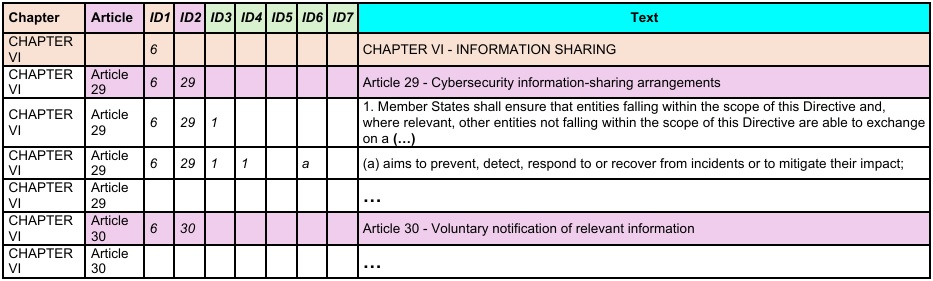
\includegraphics[width=1\textwidth]{Images/TraceMatrix.jpg} 
    \caption{Sample from the traceability matrix of \ac{NIS2} from the previous work.\cite{Pbol}}
    \label{tab:traceMatrix}
\end{figure}

% #############################################################################
\subsection{Archimate Index}

Secondly, the ArchiMate Index builds on the traceability matrix to establish an entry point, in ArchiMate, for each \ac{AD}. This establishes the ``Index'' view.
The ``Index'' view enables internal navigation between chapters and articles of the legislation and their corresponding architectural representations from a single location \cite{Pbol}.
In the ``Index'' view, each chapter of the legislation is represented as an ArchiMate group, which contains the corresponding ArchiMate views that model each legislation article. Most articles have a view that represents them, however, some were combined into a single view, subdivided across multiple views, or integrated into other related views. These variations are easily understandable due to the numbering system found within the documentation of each view element, which contains an \ac{ID} that can be traced to the corresponding legal clause using the traceability matrix.
Some views do not directly correspond to specific articles but serve either a complementary function or represent a practical scenario. These views are marked in contrasting colours to differentiate them from article-specific views. \textbf{Pink} represents practical scenarios and \textbf{yellow} depicts complementary views.
An example of the index view can be observed bellow in figure \ref{fig:nis2IndexView}

\begin{figure}
  \centering
  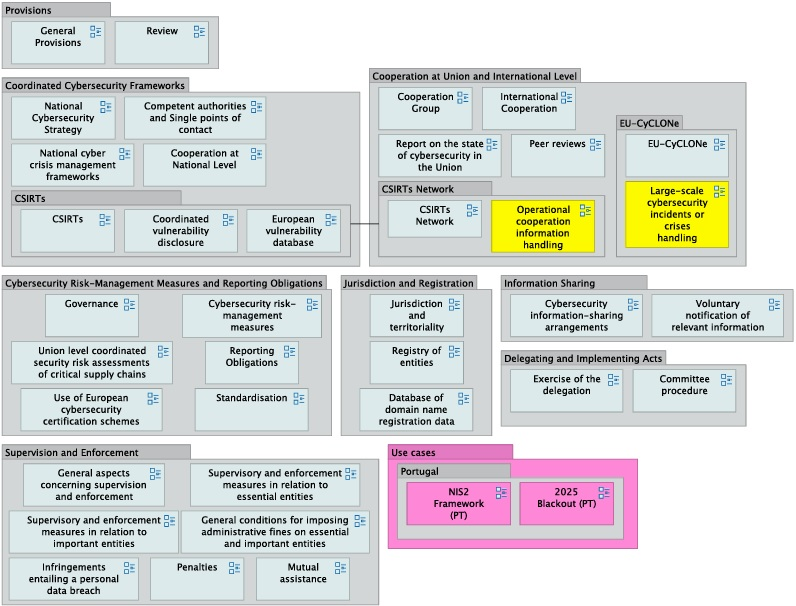
\includegraphics[width=0.8\textwidth]{Images/IndexView.jpg}
  \caption{ArchiMate \ac{NIS2} Index View from the previous work\cite{Pbol}}
  \label{fig:nis2IndexView}
\end{figure}

% #############################################################################
\subsection{Numbering System}

The Numbering system is what enables traceability across the legislation, the traceability matrix and the elements in the \ac{AD}. By providing a simple \ac{ID} mapping between the \ac{AD}'s elements and the legislation clauses listed in the matrix, it is simple to trace elements to legislative acts. 
In greater detail, the traceability matrix assigns a unique hierarchical \ac{ID} to each clause of the legislation. Each \ac{ID} level corresponds to a structural layer in the legislation.
``For instance, the clause ``Article 2, (2), (a), (i)'' might appear straightforward in the legislation, but in the matrix, it is represented as ``1.2.2.1.1.a.i'' rather than ``1.2.2.a.i''. This is because the matrix captures every intermediate level, including numbered lists or grouping structures that are sometimes implicit in the original text. In this case, ``1.2.2'' represents Chapter I, Article 2, paragraph 2. The additional ``1.1'' accounts for nested list levels within that paragraph before reaching point (a), and ``i'' represents the sub-point.''\cite{Pbol}
Cases where an element is associated with more than one \ac{ID} exist, meaning that such element is associated with more than one clause or article. Special cases of this include the wildcard, as in ``1.1.*'', denoting all sub-clauses, and ``1.-.1'' indicating the absence of a Section.

% #############################################################################
\subsection{Constructing the Architecture Descriptions}

Lastly, the method finalizes with the development of the \ac{AD}s for the specified regulation for both \ac{NIS2} and \ac{eIDAS2}. This was done by adopting a top-down approach that transitions from a high-level legislative perspective to a detailed technical modelling. Each piece of legislation underwent a comprehensive chapter-by-chapter and article-by-article analysis to identify elements relevant to the architecture, all the while prioritizing the business layer of ArchiMate to capture how the regulations impact organizational operations, roles and processes.

In order to maintain clarity and interpretive accuracy across complex legal structures, four core principles guided the development of the \ac{AD}s:

\begin{itemize}
    \item \textbf{Abstraction:} Views are maintained at a level of detail that avoids unnecessary complexity, ensuring stakeholders can focus on relevant legal requirements without becoming overwhelmed;
    \item \textbf{Reuse:} Coherence is achieved by consistently reusing defined legal elements, style types, and architecture patterns, such as event-driven or process-driven designs, throughout both \ac{AD}s to reduce duplication of effort;
    \item \textbf{Traceability:} A cornerstone of the methodology, the numbering system links every element in the ArchiMate models back to its specific legal clause in the traceability matrix, enabling verification and easier maintenance;
    \item \textbf{Modularity:} The \ac{AD}s are designed to be independent; each view typically corresponds to a single article or legal unit. This allows stakeholders to understand specific areas in isolation without having to navigate the entire repository.
\end{itemize}

Each element in the \ac{AD} is documented with references to official legislative sources. This documentation provides essential context for the independent views, ensuring that important nuances are captured and reducing the need to constantly cross-reference the original legislation or matrix.

To manage the complexity of legal modelling and support iterative refactoring, version control was integrated into the Archi tool using the coArchi2 plugin. This tool integrates Git-based functionality directly into the modelling environment, allowing for the tracking of changes and comparison of modifications.

% #############################################################################
\subsection{Results from Application to NIS2 and eIDAS2}

The application of the method to the \ac{NIS2} and \ac{eIDAS2} resulted in \ac{AD}s that are comprehensive, coherent and navigable representations of both legislations. These are made up of more than a hundred views and over a thousand numbered elements.

The \ac{NIS2} \ac{AD} focuses on operationalizing cybersecurity obligations for essential and important entities, national \ac{CSIRT}s, and European-level cooperation institutions, while the \ac{eIDAS2} \ac{AD} models the expanded legal and technical scope introduced by the revision on the original eIDAS. It covers the legal framework for digital identity, including its means, methods and mechanisms for secure identification, authentication and trust services across the \ac{EU}.

The viewpoints produced by this work are demonstrable, but they were not formally validated, resorting to \ac{GenAI} on the issue of validation.

This work explored the use of \ac{GenAI} to support the validation and documentation of complex \ac{AD}s, resorting to \ac{LLM}s such as ChatGPT and an AI-enhanced JArchi integration with LLaMA and Gemini. This exploration does not aim to replace formal validation, but rather position \ac{GenAI} as a method supporter and stressor.
To achieve this, two primary approaches where explored:

\begin{itemize}
    \item \textbf{Unit-Based Review with ChatGPT 5:}  In this approach, small ``units'' of the \ac{AD}, such as views linked to a single article, were selected and provided to the \ac{LLM} together with their traceability information and context. This context included ArchiMate XML, relevant legal text, traceability matrices and a list of tasks to perform. ChatGPT 5 successfully captured the essence of views provided in this manner and generated a positive output regarding given tasks. A very accurate clause-to-element table was generated, containing only a minor misalignment. Generated validity assessments also provided useful insights, such as the identification of missing legal provisions, and good feedback on view layout and readability was also offered.
    \item \textbf{AI-enhanced JArchi Integration:} JArchi is a JavaSript-based scripting extension for the Archi tool that allows for the customization of ArchiMate modelling tasks through JavaScript. To exploit it's potential with \ac{LLM}s, two complementary approaches were integrated:
    \begin{itemize}
        \item \textbf{LLaMA 3.1 (Documentation Augmenter):} LLaMA `` effectively demonstrated its value as a supportive assistant rather than a substitute for the expertise of the architect''\cite{Pbol}. This is due to post-editing being necessary on the generated output, such as ``aligning with the legal provisions, filtering unnecessary information, and correcting misalignments or digressions''\cite{Pbol}.
        \item \textbf{Gemini (Validation Critique):} Gemini was used to generate a validation ``critique'' of a selected view. Overall, good comments were generated suggesting more critical improvements, identifying possible omission and layering inconsistencies directly within ArchiMate.
    \end{itemize}
\end{itemize}

It is important to note that this is only a very short summary of an entire masters thesis, and only the points considered to be the most relevant for this work were covered. Many more lower level details can be found on both methodology and results in the thesis ``Conceptual Modelling of Legal Compliance Requirements - The cases of eIDAS2 and NIS2''. 

